\documentclass[a4paper,man,natbib]{apa6}
%\usepackage[square]{natbib}
\usepackage{microtype}
\usepackage{mathtools} % needed
\usepackage{hyperref}
%\usepackage{stmaryrd} % not needed
\usepackage{tabularx}
\newcolumntype{Y}{>{\raggedright\arraybackslash}X}

\usepackage[normalem]{ulem}
%\linespread{1.3}
% use apa defaults
\hypersetup{hidelinks=true}
% let's not be garish
\usepackage{lingex} % some linguistic-style example numbering


\newcommand*{\smex}[1]{\textit{#1}} % 'small example'
\newcommand*{\spex}[1]{``{#1}''} % 'spoken example'
\newcommand*{\term}[1]{\emph{#1}} % introducing a new term
\newcommand*{\citegen}[1]{\citeauthor{#1}'s~(\citeyear{#1})}
\newcommand*{\SE}{\mathit{SE}} % fix funny "SE" spacing
\newcommand{\resultsLog}[3]{$\beta = #1$, $\textnormal{SE} = #2$, $p #3$}
\newcommand{\resultsLM}[3]{$\beta = #1$, $\textnormal{SE} = #2$, $t #3$}




\title{`nervous' gestures influence listeners' online pragmatic judgments}
\author{order(Martin Corley, Josiah P.\@ J.\@ King, Jia E.\@ Loy)}
\affiliation{Psychology, PPLS, University of Edinburgh}
\ifapamodeman{\note{\begin{flushleft}%
Josiah King\\
Philosophy, Psychology and Language Sciences\\
University of Edinburgh\\
7~George Square\\
Edinburgh EH8~9JZ, UK\\[1ex]
\url{J.P.J.King@sms.ed.ac.uk}
\end{flushleft}}}




\shorttitle{gesture cues deception (GCD)}

\abstract{Previous research shows links between body language and perceptions of deception. 
Traditionally, this is considered to stem from a form of speaker-modelling: lying takes cognitive effort, and effort is associated with certain motor actions (head-scratch).
Recently, work has highlighted how listeners' associations of manner of spoken delivery (speech disfluency) with dishonesty happen at the earliest stages of reference comprehension.
Can/do listeners also rapidly integrate the visual channel in making these pragmatic judgments?

To investigate this, we look at the time-course of listeners' gesture-lying biases.
Participants saw and heard a potentially dishonest speaker describe treasure being hidden behind a named object, while also viewing both the named object and a distractor object. 
Their task was to click on the object behind which they suspected the treasure to actually be hidden.
In line with previous work, offline responses patterned with a gesture-lying bias: Participants clicked on the distractor more when they saw a video displaying the speaker producing a nervous gesture.
Importantly, this effect corresponded to an early fixation bias. 
Not only does this show the online nature of listeners' pragmatic judgments of deception, it also suggests that they are able to process and integrate gestural information in making these judgments.

incl. something about perception of nervousness - haven't looked at ratings yet, will be in expt. 2

}


\begin{document}
\maketitle
\noindent





%JK INTRO. 




%	GCD v1
\section{Experiment 1.}
The present study adapts the ‘treasure-game’ paradigm (Loy et al., 2016), in which participants make judgments about the veracity of utterances to include visual information about the speaker. 
Previous research (Vrij, 2000) suggests that listeners are more likely to make an offline judgment of an utterance as dishonest when the speaker has made a trunk movement/postural shift. 
An eye- and mouse-tracking experiment investigates whether, when a participant is making a judgment about the honesty of an utterance, the presence of a trunk movement influences the online pragmatic judgment made about the veracity of an utterance.

\subsection{Materials}
\paragraph{images}
%JK reword - stolen from Jia.
“Visual stimuli comprised 120 line drawings from Snodgrass and Vanderwart (1980), presented in pairs across sixty trials (20 critical; 40 filler). 
For each pair presented in a visual display, we will use the term referent for the object that the speaker named as the object concealing the treasure; we will refer to the other object as the distractor. 
Critical referents and distractors were matched for ease of naming (H value < 1.0) and familiarity (>=3.0) to minimize participants’ biases toward either object based on expectations relating to difficulty of description. 
Care was also taken to ensure both objects did not start with the same sound on critical trials.” (Loy et al., 2016, p 9).
\paragraph{audio}
Each referent was associated with a recording specifying the image as the object that the treasure was hidden behind (“The treasure is behind the <referent>”).
\paragraph{Video}
20 critical videos (10 Gesture, 10 No-gesture) were recorded. For the critical gesture videos, the speaker made a trunk movement, for the no-gesture videos, the speaker sat motionless.
Additionally, there were 40 filler videos (20 gesture, 20 no-gesture). 
For the filler gesture videos, 10 involved various adapter gestures (finger tapping, head tilt, etc) and 10 were of the speaker sitting motionless but in a different position to that of the no-gesture videos (hand on chin, arms crossed, etc). 

The 20 critical referents were counterbalanced across two lists, each containing 10 gesture videos, and 10 no-gesture videos, such that each referent that occurred with a gesture video in the first list occurred with a no-gesture video in the second.
So that videos could be counterbalanced across referents, and thus across utterances, the face of the speaker was blurred. 
This meant that, when presented with a given utterance, it was believable that both audio and visual stimuli had been produced concurrently. 

For each video in the gesture condition, the frame at which the gesture ended was identified, and was the point at which the utterance begins. 
Because we controlled the speech/gesture overlap (no overlap), and because gestures varied in length, the amount of video displayed prior to utterance varied (Mean = 1540ms, sd=475ms).
To control for any effect of gesture being explained a simply a sensitivity to duration of pre-utterance video, utterances in the no-gesture condition were matched to begin at the same distribution of times.

\subsection{Procedure}
Stimuli were displayed on a 21~in.\@ CRT monitor, placed 850~mm from an Eyelink~1000 Tower-mounted eye-tracker which tracked eye movements at 500~Hz (right eye only). 
Audio was presented in stereo from speakers on either side of the monitor. 
Mouse coordinates were sampled at 20~Hz. 
The experiment was presented using OpenSesame version~3.1 \citep{Mathot2012}.

Participants were told that they were going to watch videos which were recorded from a previous experiment, in which one participant had to deceive another as to the location of some hidden treasure. 
Figure \ref{fig:v1trial} presents a sample trial from the experiment. 
\begin{figure}[Ht]
  \centering
	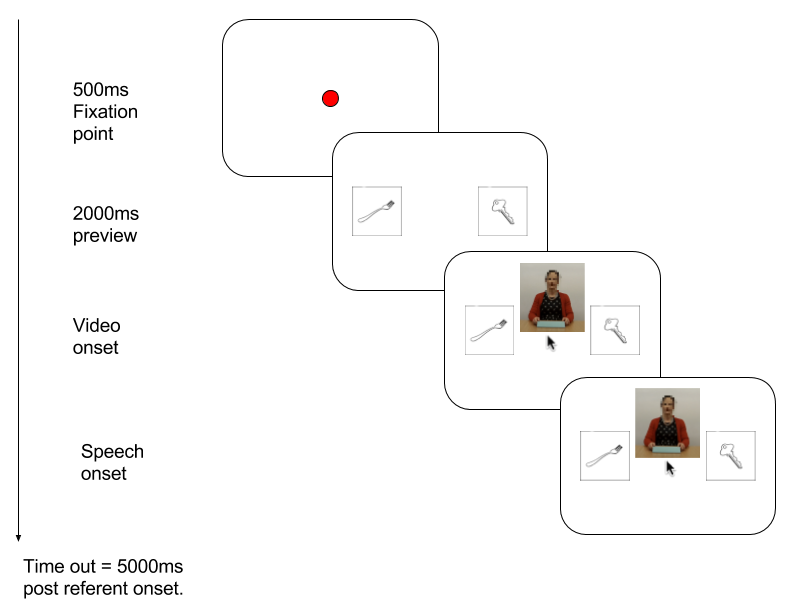
\includegraphics[width=\linewidth]{gcdv1.png}
  \caption{Procedure of a given trial.}
  \label{fig:v1trial}
\end{figure}
Between trials, participants underwent a manual drift correct, after which the fixation dot turned red for 500ms. 
The two objects (referent and distractor) were displayed on the screen for 2000ms.
After this, the video appeared and the cursor was centred and made visible. 
After either the speaker had made a trunk movement, or the equivalent time had passed (M=1540ms, sd=475ms), the utterance began. 

\paragraph{bonus rounds}
%JK DID WE USE BONUS ROUNDS? CHECK? I THINK WE DID!
To maintain motivation throughout the study, participants were told that there were a number of ``hidden bonus rounds'' which offered more treasure. 
Following 25\% of the filler trials, a ``bonus round'' message appeared before progressing to the next trial.
This informed participants that they had successfully located bonus treasure (regardless of the object chosen).
Participants were also told that the top scorers would be able to enter their names on a high-score table, which was shown at the beginning of the experiment. 

Participants completed five practice trials (one of which was presented as a bonus round) prior to the main experiment. 
Eye movements, mouse coordinates and object clicked (referent or distractor) were recorded for each experimental trial.


\paragraph{post test qs}
Participants were asked to complete a short post-test questionnaire (found on the OSF page). 
The questionnaires contained three questions, the most important of which asked if participants noticed anything odd about the visual or audio stimuli.
Any participant who indicated that they noticed anything unusual was then verbally questioned, to decide whether they believed that the speech and gesture had been produced naturally and simultaneously.
All participants were be subsequently debriefed (and told that the audio and video were created separately and stitched together), and asked again (verbally) if they noticed anything unusual. 


\subsection{Analysis}

Analysis was carried out in R version~3.3.3 \citep{rbase}, using the lme4 package \citep{lme4}. 
Trials in which participants did not click on either the referent or distractor (0.3\%) were excluded from all analyses. 

Analyses for both eye and mouse movements were conducted over a time window of 1000~ms from the 200~ms after onset of the referent name.
This window exceeds the duration of the longest critical referent name (776~ms) and is consistent with evidence that eye movements reflect the establishment of reference around 400-800~ms after noun onset \citep{Eberhard1995}.
Eye fixation data was averaged into 20~ms bins (of 10 samples) prior to analysis.
For each bin, we calculated the proportions of time spent fixating referent or the distractor, resulting in a measure of the proportions of fixations on either object over time.

The position of the mouse was sampled every 20~ms, corresponding to one bin of eye-tracking data.
Using the $X$ coordinates only, we calculated the number of screen pixels moved and the direction of movement (towards referent or distractor).
The cumulative distance traveled towards each object was calculated for each bin, and divided by the total distance moved, regardless of direction.
The resulting measure was the proportion of total distance traveled towards either object over time.
%JK Trials for which the total mouse distance traveled post referent-onset was less than one third of the distance from the screen center to the near edge of an object were excluded (???\% of trials). 
%JK Movements beyond the outer edge of either object were considered to be `overshooting' and were not included in calculations (???\% of samples).

We used an empirical logit transform to measure relative biases in eye and mouse movements \citep{Barr2008}.
Eye movement biases were calculated from the proportions of referent to distractor fixations;
mouse movement biases were calculated analogously.
A value of zero in either measure indicates no bias towards either object, and positive and negative values indicate a bias towards the referent and distractor respectively.

%JK WHAT ARE WE DOING RE: analysis of v1? looking at fillers or no? 
Linear mixed effects models of eye and mouse movements included fixed effects of time, gesture and their interactions.
Random intercepts and slopes for time and gesture were included by-participant and by-referent.
Following \citet{baayen2008analyzing}, we considered effects in these models to be significant where $|t|>2$.

The object clicked (referent or distractor) was modeled using mixed effects logistic regression.
This model included  fixed effects of gesture with random intercepts and slopes for gesture by-participant and by-referent.

\subsection{results}
\subsubsection{Object click}
\subsubsection{Eye movements}
\subsubsection{Mouse movements}

\subsection{Discussion}











% GCD v2
\section{Experiment 2.}
%JK summarise differences/motivations
same as experiment 1 only reduced set (no filler trials), constant speech onset latency, just adaptor gesture, 

There were several things to note from version 1. 
Firstly, the gestures used in the filler trials (adaptor gestures, often involving hands) appeared to bias participants more strongly towards an eventual interpretation of dishonesty than the critical gestures (trunk movements). 
This could be simply that the filler gestures were more visually salient than trunk movements, resulting in participants attending towards the speaker’s hands more than to her trunk.
Alternatively, it could be that listeners do not associate trunk movements with deception, contra previous research (Vrij, 2000)

Several participants reported post-test that in making their judgments, they were assessing “how relaxed” the speaker looked during the utterance. 
This led us to rethink our justification for the type of gesture which we would expect to elicit judgments of dishonesty. 
In the current version (version 2) we make the following line of reasoning: If listeners are reasoning (perhaps via introspection) about what lying involves (e.g. effort, nervousness, etc.), then gestures which are likely to function as cues to deception should reflect this  reasoning.

An additional comment from several participants was that they sometimes considered the no-gesture videos to show the speaker looking more unrelaxed.
This is something we had not considered, and we attempted to make the no-gesture videos for version 2 look more relaxed (more slumped/slouched posture).

Based on Gregerson (2005), we use adaptor gestures as our critical gestures. 
Adaptors are typically associated with nervousness, and include various hand and arm gestures such as finger taps, fidgeting, rubbing shoulders etc. 

Additionally, all videos are rated by 10 naive volunteers for “how nervous the speaker looks” prior to running the study.
Post-test, participants will be asked to rate a selection of videos (both gesture and no-gesture) for nervousness.
Key differences between version 1 and version 2.
Version 2 contains no filler trials.
Version 1 contained 40 filler trials with various gestures, which in hindsight served no purpose. In fact, they contained the very types of gesture which are likely to be a) more salient and b) more strongly associated with lying (given an introspection speaker modelling account).
Version 2 = 20 trials long. Practice trials changed from 5 to 4.

Critical gestures are adaptors (as opposed to trunk movements in version 1)
A result of this is that in version 2 there is gesture/speech overlap, whereas in version 1 there was no overlap. This might cause problems as participants may fixate more to the gesturing than to the objects at the relevant time (referent onset).
No-gesture videos show the speaker in a more relaxed posture.
All videos rated (n=10) for nervousness prior to study.
Video onset to speech onset is a constant (rather than a variable matched across conditions)
Participants rate videos for nervousness post-test.


\subsection{Materials}
%images
%JK same as crit from v1
Visual stimuli comprised 40 line drawings from Snodgrass and Vanderwart (1980), presented in pairs across twenty trials. For each pair presented in a visual display, we will use the term referent for the object that the speaker named as the object concealing the treasure; we will refer to the other object as the distractor. Critical referents and distractors were matched for ease of naming (H value < 1.0) and familiarity (>=3.0) to minimize participants’ biases toward either object based on expectations relating to difficulty of description. Care was also taken to ensure both objects did not start with the same sound on critical trials. (Loy et al., 2016).

%audio
%JK same as crit from v1
Each referent was associated with a recording specifying the image as the object that the treasure was hidden behind (“The treasure is behind the <referent>”).

%Video
20 videos (10 Gesture, 10 No-gesture) were used.
The 10 videos in the gesture condition showed the speaker making some form of adaptor gesture (tapping fingers, twirling hair, rubbing shoulder, etc).
The 10 no-gesture videos showed the speaker sitting motionless. 

%lists
The 20 critical referents were counterbalanced across two lists, each containing 10 gesture videos, and 10 no-gesture videos, such that each referent that occurred with a gesture video in the first list occurred with a no-gesture video in the second.
So that videos could be counterbalanced across referents, and thus across utterances, the face of the speaker was blurred. This meant that, when presented with a given utterance, it was believable that both audio and visual stimuli had been produced concurrently. 
To allow time for gesture to be fully initiated, the video is displayed 1170ms prior to utterance onset. 

\subsection{Norming}
All videos were rated on how nervous the speaker looked on a scale of 1 to 7, with 1 being very relaxed and 7 being very nervous.
10 native english speakers watched the videos and asked: “These are videos (without audio) of someone being questioned in a stressful situation. Rate on a scale of 1 to 7 on how nervous they look in each video. 1 = very relaxed, 7 = very nervous.”.
The gesture videos were rated as more nervous (mean = 4.1, sd = 1.5) than the no-gesture videos (M = 1.9, sd = 1.1).

\subsection{Procedure}
%JK same as epxeriment 1 only constant speech onset time.
Participants were told that they are going to watch videos which were recorded from a previous experiment, in which one participant had to deceive another as to the location of some hidden treasure. 
Figure \ref{fig:v2trial} presents a sample trial from the experiment. 
\begin{figure}[Ht]
  \centering
	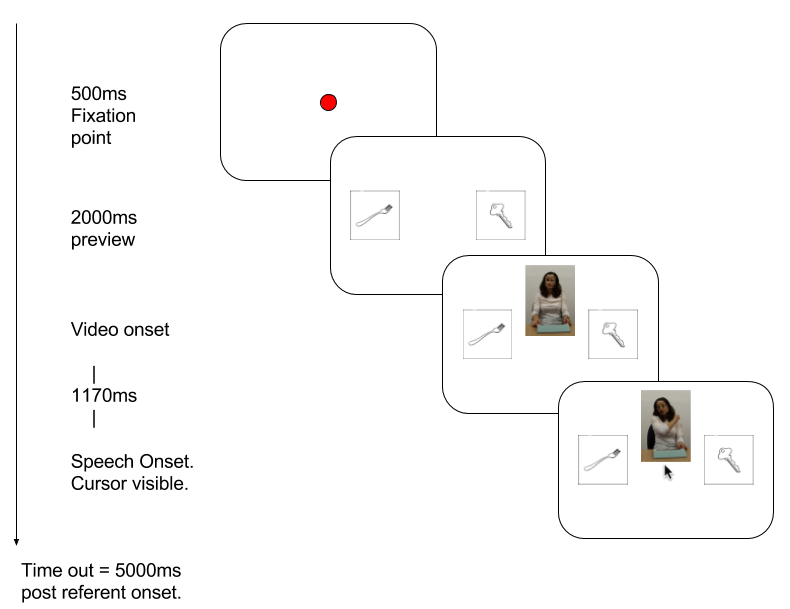
\includegraphics[width=\linewidth]{gcdv2.png}
  \caption{Procedure of a given trial.}
  \label{fig:v2trial}
\end{figure}
Between trials, participants undergo a manual drift correct, after which the fixation dot turns red for 500ms. 
The two objects (referent and distractor) are displayed on the screen for 2000ms.
After this, the video appears and the cursor is centred and made visible. 
After 1170ms the utterance begins. 

\subsection{post-test qs}
%JK same as exp. 1
Participants are asked to complete a short post-test questionnaire (found on the OSF page). 
The questionnaires contain three questions, the most important of which asks if participants noticed anything odd about the visual or audio stimuli.
Any participant who indicates that they noticed anything unusual will then be verbally questioned, to decide whether they believed that the speech and gesture had been produced naturally and simultaneously.
All participants will be subsequently debriefed (and told that the audio and video were created separately and stitched together), and will be asked again (verbally) if they noticed anything unusual. 


\subsection{Analysis}
%JK same as for v1
%JK what about the ratings?

\subsection{results}
\subsubsection{Object click}
\subsubsection{Eye movements}
\subsubsection{Mouse movements}

\subsection{gen. discussion}


\end{document}
